\chapter{Services}
\label{chp:services}
De tweede manier van communicatie tussen nodes in ROS zijn \textit{services}. Services werken met een \textit{call-and-response}-model. Dit betekent dat er alleen een bericht/informatie/data wordt gegeven als er om wordt gevraagd. Dit is een groot verschil met topics. Bij topics worden er constant updates gegeven op de topic ongeacht of iemand er om vraagt. Het initiatief bij een topic ligt bij de publishers.

Bij services hebben we \textit{clients}, die om informatie kunnen vragen, en een \textit{server} die na aanvraag van een client de informatie levert. Het initiatief van de communicatie ligt bij de clients. Een service kan meerdere clients hebben, maar een service kent altijd maar \'e\'en server. In figuur \ref{fig:service} zien we een voorbeeld van een services met \'e\'en server en twee clients. Node 1 zal pas een \textit{response} geven, nadat het een \textit{request} heeft ontvangen van node 2 of 3.

\begin{figure}[ht] % ’ht’ tells LaTeX to place the figure ’here’ or at the top of the page
\centering % centers the figure
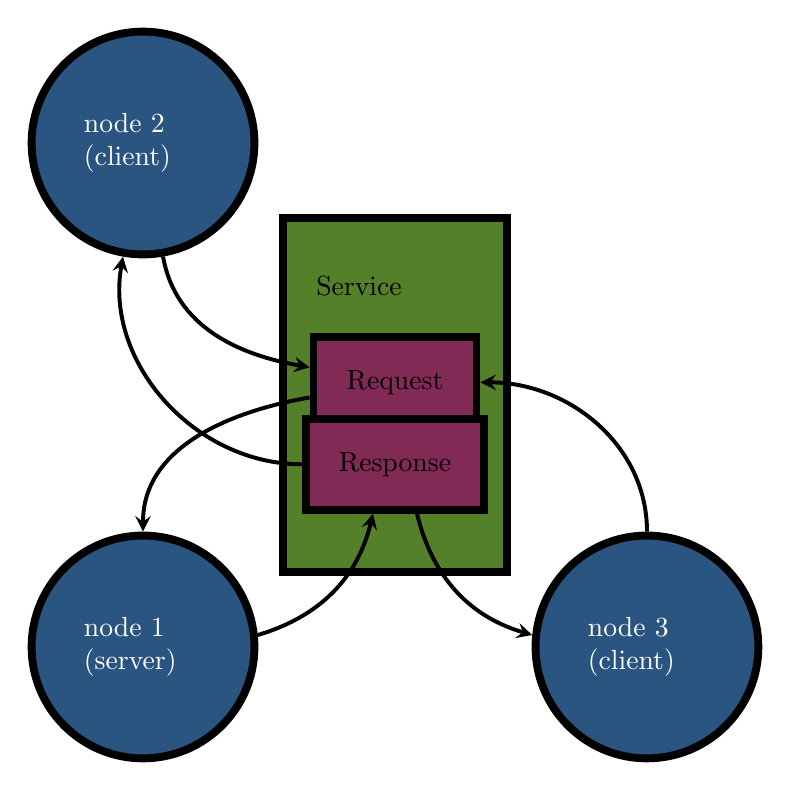
\begin{tikzpicture}[->, >=stealth, node distance=4cm, line width=1mm, scale=0.8]
\node[circle, draw=black, fill={rgb:red,1;green,2;blue,3}, inner sep=12pt, minimum size=12pt, , text width=1.5cm] (A) at (0,0) {\textcolor{white}{node 1 (server)}};
\node[circle, draw=black, fill={rgb:red,1;green,2;blue,3}, inner sep=12pt, minimum size=12pt, text width=1.5cm] (B) at (0,8) {\textcolor{white}{node 2 (client)}};
\node[circle, draw=black, fill={rgb:red,1;green,2;blue,3}, inner sep=12pt, minimum size=12pt, text width=1.5cm] (C) at (8,0) {\textcolor{white}{node 3 (client)}};
\node[rectangle, draw=black, fill={rgb:red,2;green,3;blue,1}, inner sep=12pt, minimum height = 4.5cm] (service) at (4,4) {\begin{minipage}[t][3cm]{2cm}Service\end{minipage}};
\node[rectangle, draw=black, fill={rgb:red,3;green,1;blue,2}, inner sep=12pt] (request) at (4,4.2) {Request};
\node[rectangle, draw=black, fill={rgb:red,3;green,1;blue,2}, inner sep=12pt] (response) at (4,2.9) {Response};

\draw [->, line width=0.5mm, bend right]  
            (A) edge (response) 
            (response) edge (C);
\draw [->, line width=0.5mm]            
            (response) to[out=180,in=-100, ->] (B);
\draw [->, line width=0.5mm]            
            (C) to[out=90,in=360] (request) ;
\draw [->, line width=0.5mm]            
            (B) to[out=-80,in=170] (request) ;
\draw [->, line width=0.5mm]            
            (request) to[out=190,in=90] (A) ; 

\end{tikzpicture}
\caption{Een ROS service. Met node 1 als server en node 2 en 3 als client.}
\label{fig:service}
\end{figure}

\section{Request and response structure}
\label{sec:srv_messages}
Een service heeft altijd een request and response structure beschreven in bestand van het type \textit{.srv}. In deze structuur staan de parameters van het request en het de response van de service. De parameter(s) van de request staan boven een streep van drie gedachtestreepjes (---)\footnote{Het gedachtestreepje of aandachtsstreepje is een leesteken dat de vorm heeft van een liggend streepje. Zie ook: \url{https://nl.wikipedia.org/wiki/Gedachtestreepje}}. De parameter(s) van de response staan onder de drie gedachtestreepjes. In codevoorbeeld \ref{code:AddThreeInts_srv_msg} zien we een voorbeeld van een request and response structure. De request bestaat in dit voorbeeld uit de drie parameters \textit{a}, \textit{b} en \textit{c} van het type int64 en de response bestaat uit de parameter \textit{sum} van het type int64. 

\begin{lstlisting}[language=C++, caption={AddThreeInts.srv}, firstnumber=0, label={code:AddThreeInts_srv_msg}]
int64 a
int64 b
int64 c
---
int64 sum
\end{lstlisting}

\noindent De mogelijke types die kunnen worden gebruikt in de request and repsonse structure zijn te vinden op:
\begin{center}
    \url{https://index.ros.org/doc/ros2/Concepts/About-ROS-Interfaces/}
\end{center}

\noindent Net zoals het message type van de publishers/subscribers (zie sectie \ref{sec:message_types}) is het mogelijk de request and response structure binnen de package te plaatsen, maar ook om deze buiten de package te plaatsen. 

\noindent \textbf{Let op:} Bij het maken van een \textit{.srv}-bestand is het verplicht in de naamgeving PascalCase\footnote{zie \url{https://nl.wikipedia.org/wiki/CamelCase}} te gebruiken. ROS zet de \textit{.srv} om naar een \textit{.hpp}-bestand met de naam in snake\_case \footnote{zie: \url{https://en.wikipedia.org/wiki/Snake_case}}, waarbij tussen elke kleine letter en hoofdletter van de PascalCase naamgeving nu een onderstrepingsteken (\_)\footnote{ook wel bekent als \textit{underscore}. Zie \url{https://nl.wikipedia.org/wiki/Underscore}} staat. Bijvoorbeeld de request and response structure beschreven in \textit{MyCustomService.srv} wordt geïncludeerd met: 
\begin{lstlisting}[language=C++, caption={}, firstnumber=0, label={}]
#include "path/to/folder/my_custom_service.hpp".
\end{lstlisting}

Zie sectie \ref{sec:service_andere_bronnen} voor verwijzingen naar bronnen die met meer diepgang messages en request and response structures van ROS behandelen. In deze bronnen staat ook hoe je .srv-bestanden toevoegd aan je package en hoe je ze vanuit een andere package includeert.

\section{Server code}
Een node noemen we een \textit{service}, \textit{server} of, om extra onderscheid te maken met een \textit{action server} (zie hoofdstuk \ref{chp:actions}), een \textit{service server} als het een membervariabele van het type \textit{rclcpp::Service<T>} heeft. Een rclcpp::Service<T> is een template-class die een request and response structure nodig heeft. Het declareren van een rclcpp::Service<T> variabele doen we binnen de node met \textit{rclcpp::Service<request\_response\_structure>::SharedPtr service\_name;}. Bijvoorbeeld de server \textit{service\_} met de request and response structure \textit{myPackages/srv/MyStruct.srv}\footnote{Zie sectie \ref{sec:srv_messages}}:
\begin{lstlisting}[language=C++, caption={Een voorbeeld van het declareren van een service server.}, firstnumber=0, label={}]
#include "myPackages/srv/my_struct.hpp"
// [...]
rclcpp::Service<myPackages::srv::MyStruct>::SharedPtr service_;
\end{lstlisting}

Een service reageert op elk bericht. Bij het initialiseren van de service moeten we daarom net als bij de subscriber een functie toekennen die het bericht afhandelt. Deze functie heeft verplicht twee parameters: een shared pointer naar de request en een shared pointer naar de response. Hiermee kan de functie de data van de request binnen krijgen en met de response kan de service data terugsturen naar client. Het toekennen van de functie aan de service doen we met \textit{create\_service<T>()} die we erven van de superclass rclcpp::Node. De functie \textit{create\_service<T>()} verwacht, naast een binding met een functie, de naam van de service en een request and response structure. In het geval van de bovenstaand gedeclareerde \textit{service\_} met de service naam ``my\_service'' en de member functie \textit{provideService()} die de service-request afhandelt doen we dat met:

\begin{lstlisting}[language=C++, caption={Het initialiseren van een service server. Meestal gebeurt dit in de constructor.}, firstnumber=0, label={}]
#include "myPackages/srv/my_struct.hpp"

using std::placeholders::_1;
using std::placeholders::_2;
// [...]
service_ = this->create_service<myPackages::srv::MyStruct>(
            "my_service", 
            std::bind(&myNode::provideService, this, _1, _2));
\end{lstlisting}

De \textit{std::placeholders} moeten we in de \textit{std::bind()} gebruiken omdat we een placeholder moeten geven voor de twee parameters die de gekoppelde functie verplicht moet hebben\footnote{Een uitleg over \textit{std::bind} en \textit{std::placeholders} kan men vinden op: \url{https://www.youtube.com/watch?v=JtUZmkvroKg}}. De functie die gekoppeld is aan de service heeft verplicht twee parameters: request en response. De types van de parameters zijn afhankelijk van het .srv-bestand, maar zijn altijd een shared pointer. De gekoppelde functie heeft als taak een response te bepalen, eventueel aan de hand van het request, en deze toe te kennen aan de response parameter. Codevoorbeeld \ref{code:service-server-function} geeft een voorbeeld van een dergelijke functie. Het voorbeeld gebruikt de request and response van codevoorbeeld \ref{code:AddThreeInts_srv_msg}.

\begin{lstlisting}[language=C++, caption={Een voorbeeld van een service-functie.}, firstnumber=0, label={code:service-server-function}]
void myNode::provideService(
    const std::shared_ptr<srvcli_custom_srv_in_pkg::srv::AddThreeInts::Request> request,
    std::shared_ptr<srvcli_custom_srv_in_pkg::srv::AddThreeInts::Response> response )
{
  // processing the request (calculating the sum) and assigning it to the response:
  response->sum = request->a + request->b + request->c;
}
\end{lstlisting}

\noindent In codevoorbeelden  \ref{code:server_hpp},  \ref{code:server_cpp} en \ref{code:server_main} zien we alle serveronderdelen samengevoegd tot de server node \textit{ServiceNode}. ServiceNode maakt gebruikt de request and response structure gedefineerd in codevoorbeeld \ref{code:AddThreeInts_srv_msg}. De node is ook te vinden de package-voorbeelden die komen met deze reader.

\begin{lstlisting}[language=C++, caption={ServiceNode.hpp}, firstnumber=0, label={code:server_hpp}]
#include "rclcpp/rclcpp.hpp"
// srv/AddThreeInts.srv becomes srv/add_three_ints.hpp:
#include "srvcli_custom_srv_in_pkg/srv/add_three_ints.hpp"

class ServiceNode : public rclcpp::Node
{
public:
  ServiceNode();
  
private:
    // function to be called by the service.
    void add(
    const std::shared_ptr<srvcli_custom_srv_in_pkg::srv::AddThreeInts::Request> request,
    std::shared_ptr<srvcli_custom_srv_in_pkg::srv::AddThreeInts::Response> response
    );

    rclcpp::Service<srvcli_custom_srv_in_pkg::srv::AddThreeInts>::SharedPtr service_;
};
\end{lstlisting}


\begin{lstlisting}[language=C++, caption={ServiceNode.cpp}, firstnumber=0, label={code:server_cpp}]
#include "rclcpp/rclcpp.hpp"
// srv/AddThreeInts.srv becomes srv/add_three_ints.hpp:
#include "srvcli_custom_srv_in_pkg/srv/add_three_ints.hpp"
#include "ServiceNode.hpp"

// placeholders for the arguments
using std::placeholders::_1;
using std::placeholders::_2;

ServiceNode::ServiceNode(): Node("ServiceNode"){
    // initialise the service
    // <srv-message-type> in this case custom_interfaces::srv::AddTwoInts
    // "add_three_ints" the name of the topic
    // and a pointer to the function to be called when a service message is received.
    service_ = this->create_service<srvcli_custom_srv_in_pkg::srv::AddThreeInts>(
            "add_three_ints", 
            std::bind(&ServiceNode::add, this, _1, _2));
}

void ServiceNode::add(
    const std::shared_ptr<srvcli_custom_srv_in_pkg::srv::AddThreeInts::Request> request,
    std::shared_ptr<srvcli_custom_srv_in_pkg::srv::AddThreeInts::Response> response
){
  // processing the request (calculating the sum) and assigning it to the response:
  response->sum = request->a + request->b + request->c;

  // for example purposes, printing to the logging:
  RCLCPP_INFO(rclcpp::get_logger("rclcpp"), "Incoming request\na: %ld" " b: %ld" "c: %ld",
                request->a, request->b, request->c);
  RCLCPP_INFO(rclcpp::get_logger("rclcpp"), "sending back response: [%ld]", 
                (long int)response->sum);
}
\end{lstlisting}


\begin{lstlisting}[language=C++, caption={mainServer.cpp}, firstnumber=0, label={code:server_main}]
#include "rclcpp/rclcpp.hpp"
#include "ServiceNode.hpp"

int main(int argc, char **argv)
{
  rclcpp::init(argc, argv);
  rclcpp::spin(std::make_shared<ServiceNode>());
  rclcpp::shutdown();
  return 0;
}
\end{lstlisting}

\section{Client code}
Om een request in te dienen bij een ROS-service moeten we de communicatierol \textit{client}\footnote{Soms ook \textit{service client} genoemd om duidelijker onderscheid te maken met \textit{action clients}} aannemen. Dit doen we door een member variabele te declareren van het type \textit{rclcpp::Client<T>}. Een rclcpp::Client<T> is een template-class die een request and response structure (zie sectie \ref{sec:srv_messages}) nodig heeft. Het declareren van een rclcpp::Client<T> variabele doen we binnen de node met \textit{rclcpp::Client<request\_response\_structure>::SharedPtr client\_name;}. Bijvoorbeeld de client \textit{client\_} met de request and response structure \textit{myPackages/srv/MyStruct.srv}: 

\begin{lstlisting}[language=C++, caption={Een voorbeeld van het declareren van een service client.}, firstnumber=0, label={}]
#include "myPackages/srv/my_struct.hpp"
// [...]
rclcpp::Client<myPackages::srv::MyStruct>::SharedPtr client_;;
\end{lstlisting}

Voor het initialiseren van de rclcpp::Client<T> gebruiken we de functie \textit{create\_client<T>()} die een node erft van rclcpp::Node. Deze functie verreist enkel de naam van de service als argument. Het versturen van de request en het koppelen van een functie aan het ontvangen van de response handelen we later af. De initialisatie is dus relatief simpel. In het geval van de bovenstaande gedeclareerde \textit{client\_} met de service naam ``my\_service'' doen we dat met:

\begin{lstlisting}[language=C++, caption={Het initialiseren van een service client. Meestal gebeurt dit in de constructor.}, firstnumber=0, label={}]
#include "myPackages/srv/my_struct.hpp"
// [...]
client_ = this->create_client<myPackages::srv::MyStruct>("my_service");;
\end{lstlisting}

Met de geïnitialiseerde service client kunnen we nu een request sturen naar de service server. Hiervoor maken we eerst een request. Dit doen we door een shared pointer te maken van de request van de juiste request and response structure. Hiervoor gebruiken we de functie \textit{Request()} die samen met de request and response structure komt. In het geval van de request and response structure \textit{AddThreeInts.srv} (zie codevoorbeeld \ref{code:AddThreeInts_srv_msg}) doen we dat als volgt:

\begin{lstlisting}[language=C++, caption={}, firstnumber=0, label={}]
auto request = std::make_shared<srvcli_custom_srv_in_pkg::srv::AddThreeInts::Request>();
\end{lstlisting}

Voordat we de request versturen moet hij nog gevuld worden met data. De request heeft publieke member-variabelen met de namen zoals aangegeven in de request and response structure. Hieraan kunnen we direct waardes toekennen. Bij de bovenstaand gemaakte \textit{request} vullen we de drie member \textit{a}, \textit{b} en \textit{c} op de volgende manier:

\begin{lstlisting}[language=C++, caption={}, firstnumber=0, label={}]
request->a = 5;
request->b = 7;
request->c = 9;
\end{lstlisting}

Nu we een request gevuld met data hebben, kan deze worden verstuurd. Voordat we de request versturen is het verstandig om te kijken of de service server node wel aan het draaien is. Dit kunnen we doen met behulp van de functie \textit{wait\_for\_service()} van de client die we hebben gemaakt. Het volgende stuk code controleert elke seconde of de service server draait, totdat hij de server heeft gevonden. 
\begin{lstlisting}[language=C++, caption={}, firstnumber=0, label={}]
while (!client_->wait_for_service(1s)) {
    if (!rclcpp::ok()) {
        RCLCPP_ERROR(
            rclcpp::get_logger("rclcpp"), 
            "Interrupted while waiting for the service. Exiting."
        );
    }
    RCLCPP_INFO(rclcpp::get_logger("rclcpp"), "service not available, waiting again...");
}
\end{lstlisting}

Gegeven dat de service server bestaat kan er een request worden gestuurd door middel van de functie \textit{async\_send\_request()}. Deze functie van onze rclcpp::Client<T> heeft als argumenten de gemaakte request en binding met een functie die response van de server afhandelt. De functie die de response afhandelt heeft als parameter de response van de server. Met de client \textit{client\_}, de request \textit{request} en de functie \textit{handleResponse()} (met als argument de response, maar die binden we tijdelijk met een \textit{std::placeholder}), die het response van de server afhandelt, versturen we de request op de onderstaande manier:

\begin{lstlisting}[language=C++, caption={Een voorbeeld van het versturen van een request door een rclcpp::Client.}, firstnumber=0, label={code:request_versturen}]
usingstd::placeholders::_
// [...]
auto future = client_->async_send_request(request, std::bind(&ClientNode::handleResponse, this, _1));
\end{lstlisting}

\noindent de rclcpp::Client<T> biedt ook nog andere mogelijkheden rond het versturen van requests. De return value van \textit{async\_send\_request()}, in codevoorbeeld \ref{code:request_versturen} \textit{future} genoemd, biedt ook nog mogelijkheden die interessant zijn om te verkennen, maar waar we in deze reader niet op in gaan.

Met deze onderdelen kunnen we een service client node maken die een request stuurt naar de eerder genoemde service server node. Dit is uitgewerkt in codevoorbeelden \ref{code:client_hpp}, \ref{code:client_cpp} en \ref{code:client_main}. Dit voorbeeld staat ook in de voorbeelden-packages die komen bij deze reader. 

\begin{lstlisting}[language=C++, caption={ClientNode.hpp}, firstnumber=0, label={code:client_hpp}]
#include "rclcpp/rclcpp.hpp"
// srv/AddThreeInts.srv becomes srv/add_three_ints.hpp:
#include "srvcli_custom_srv_in_pkg/srv/add_three_ints.hpp"

class ClientNode : public rclcpp::Node
{
public:
    ClientNode();
  
private:
    // function that makes the request:
    void makeRequest();
    
    // function that handles the response:
    void handleResponse(rclcpp::Client<srvcli_custom_srv_in_pkg::srv::AddThreeInts>::SharedFuture future);

    rclcpp::Client<srvcli_custom_srv_in_pkg::srv::AddThreeInts>::SharedPtr client_;
};

\end{lstlisting}


\begin{lstlisting}[language=C++, caption={ClientNode.cpp}, firstnumber=0, label={code:client_cpp}]
#include "rclcpp/rclcpp.hpp"
// srv/AddThreeInts.srv becomes srv/add_three_ints.hpp:
#include "srvcli_custom_srv_in_pkg/srv/add_three_ints.hpp"
#include "ClientNode.hpp"

// needed for the use of the 's' notation in wait_for_service()
using namespace std::chrono_literals;

// placeholder for the arguments
using std::placeholders::_1;

ClientNode::ClientNode(): Node("ClientNode"){
    // initialise the client.
    // "add_three_ints" the name of the service
    client_ = this->create_client<srvcli_custom_srv_in_pkg::srv::AddThreeInts>("add_three_ints");

    // call the service:
    makeRequest();
}

void ClientNode::makeRequest(){
    // make a request of the right srv-type:
    auto request = std::make_shared<srvcli_custom_srv_in_pkg::srv::AddThreeInts::Request>();
    // add the data to the request
    request->a = 5;
    request->b = 7;
    request->c = 9;

    // wait for the service to exist.
    // if the service is never started this is a endless loop
    while (!client_->wait_for_service(1s)) {
        if (!rclcpp::ok()) {
            RCLCPP_ERROR(
                rclcpp::get_logger("rclcpp"), 
                "Interrupted while waiting for the service. Exiting."
            );
        }
        RCLCPP_INFO(
            rclcpp::get_logger("rclcpp"), 
            "service not available, waiting again..."
        );
    }

    // send the request and bind the function call the handels the response
    auto future = client_->async_send_request(
        request, 
        std::bind(&ClientNode::handleResponse, this, _1)
    );
}

void ClientNode::handleResponse(
    rclcpp::Client<srvcli_custom_srv_in_pkg::srv::AddThreeInts>::SharedFuture future
){
    auto result = future.get();
    RCLCPP_INFO(this->get_logger(), "Result of add_two_ints: %i", result->sum);
}
\end{lstlisting}


\begin{lstlisting}[language=C++, caption={mainClient.cpp}, firstnumber=0, label={code:client_main}]
#include "rclcpp/rclcpp.hpp"
#include "example_interfaces/srv/add_two_ints.hpp"
#include "ClientNode.hpp"

int main(int argc, char **argv)
{
    rclcpp::init(argc, argv);
    rclcpp::spin(std::make_shared<ClientNode>());
    rclcpp::shutdown();
    return 0;
}
\end{lstlisting}


\section{Meer bronnen}
\label{sec:service_andere_bronnen}
Andere voorbeelden van het maken van een server en een client kan men vinden in de voorbeeld-ROS-packages die komen bij deze reader of op:
\begin{center}
{\footnotesize \url{ https://index.ros.org/doc/ros2/Tutorials/Writing-A-Simple-Cpp-Service-And-Client/}} \\
\end{center}
\noindent Hoe je eigen service en message definieert kan je vinden op:
\begin{center}
    {\footnotesize \url{https://index.ros.org/doc/ros2/Tutorials/Custom-ROS2-Interfaces/}}\\
    en extra verdieping: \\
    {\footnotesize \url{https://index.ros.org/doc/ros2/Tutorials/Single-Package-Define-And-Use-Interface/}}
\end{center}

